\documentclass{article}
% Language setting
% Replace `english' with e.g. `spanish' to change the document language
\usepackage[english]{babel}

% Set page size and margins
% Replace `letterpaper' with `a4paper' for UK/EU standard size
\usepackage[a4paper,margin=0.5in]{geometry}

% Useful packages
\usepackage{amsmath,amsfonts, caption}
\usepackage{graphicx}
\usepackage{authblk}
\usepackage{float}
\usepackage[colorlinks=true, allcolors=blue]{hyperref}
\usepackage{natbib}
\usepackage{indentfirst}
\usepackage{lipsum}

\title{Estimating Somatic Variant Quality from Clonal Sequencing using Hierarchical Bayesian Models}
\author[1,*]{Arjun Biddanda}
\affil[1]{Johns Hopkins University, Department of Biology}
\affil[*]{Contact: \href{mailto:abiddan1@jhu.edu}{abiddan1@jhu.edu}}

\date{\today}

\begin{document}

\maketitle
\begin{abstract}
\lipsum[30]
\end{abstract}


\section*{Introduction}

The primary goal here is to develop a principled method to estimate the \textit{probability} that an observed clonal variant is actually somatic and not a germline variant. The core intuition used by a number of somatic variant callers is that (1) a germline variant is shared across all somatic clones and (2) is also present in a germline sample. Without loss of generality we assume that ``clone'' refers to sequencing data from a single colony derived from a blood progenitor lineage or in cases of other tissues, a laser-capture microdissection.


We specifically want to model how the germline sample, alongside additional information can provide ``prior'' information on whether a variant is likely to be polymorphic in the germline (e.g., population allele frequency). The likelihood is then defined using the collected evidence for that polymorphism across **all** of the individual clone sequences. We detail a flexible model below that can incorporate an arbitrary number of variant-level annotations for the prior probability of germline polymorphism (e.g., variant-level masks, allele frequencies, region-specific mutation rate). 


\section*{Model}

We start from a model where the output consists of diploid genotype likelihoods from each of the $J$ clonal samples at the $k^{th}$ site:

\begin{equation}
\begin{aligned}
P(GL_k | p_k) &= \sum_j^J \sum_{g\in\{0,1,2\}}P(R_j | G_j = g)P(G_j = g),
\end{aligned}
\end{equation}

, where $P(G_j = g)$ is the prior probability of a specific \textit{clonal} genotype at the $k^{th}$ site in the $j^{th}$ sample. For the purposes of 


where $f_{Z=0}(p) \sim Beta(\alpha_0, \alpha_0)$, where $\alpha_0 >> 1$  and $f_{Z=1}(p) \sim Beta(1,1)$. We should also note that in some cases there might actually be some core benefit to have $f_{Z=1}(p) ~ Beta(\alpha_1, \alpha_1)$ where $\alpha_1 < 1$.

Following this likelihood definition,  we can also focus on using annotations $\theta_k$ to help with the "prior" probability $P(Z_{k} | \theta_{k})$ , where $\theta_{k}$ represents a set of annotations for the $k^{th}$ site (e.g. germline sample genotype relative likelihood, gnomAD allele frequency, masking, local GC content, etc). We create the following logistic model for the priors based on filled annotations: 

$$
\begin{aligned}
	x_{k} &= \sum_l^L \lambda_l \theta_{kl}\\
	\pi_{k} &= P(Z_{k} = 1 | \theta_{k}, \Lambda) = \frac{1}{1 + e^{-x_{ik}}}
\end{aligned}
$$

Using this kind of prior, we can model each sites genotype likelihood as coming from a mixture of the two latent distributions:

$$P(GL | \alpha_0, \Lambda) = \prod_k^K \pi_k P(GL_k| Z_k = 1) + (1 - \pi_k)P(GL_k | Z_k = 0)$$
, where each of the $K$ sites are treated as independent realizations of this data generating process. Each iteration of this likelihood takes $\mathcal{O}(JK)$ to compute. We will then use this likelihood to estimate the hidden parameters $\hat{\Lambda}, \hat{\alpha_0}$, to inform our prior distribution.  

Armed with the parameters $\hat{\Lambda}, \hat{\alpha_0}$ we can then estimate the posterior probability of $Z_k = 1$ as: 

$$
\begin{aligned}
P(Z_k = 1 | GL_k, \theta_k, \Lambda, \alpha_0) &= \frac{P(GL_k|Z_k=1)P(Z_k=1 | \Lambda, \alpha_0)}{P(GL_k|Z_k=1)P(Z_k=1 | \Lambda, \alpha_0) + P(GL_k|Z_k=0)P(Z_k=0 | \Lambda, \alpha_0)}\\
&=  \frac{\pi_k P(GL_k|Z_k=1, \alpha_0)}{\pi_k P(GL_k|Z_k=1, \alpha_0) + (1 - \pi_k)P(GL_k|Z_k=0, \alpha_0)}
\end{aligned}
$$

This calculated posterior probability is then used as a quantitative filter for downstream VCF files. Our core argument here is that this effectively takes into account latent annotations in a way that their overall contribution to a variant being truly somatic can be estimated across the genome. The graphical model depiction below describes what is being estimated at a slightly different level as well. 


\begin{figure*}
\begin{center}
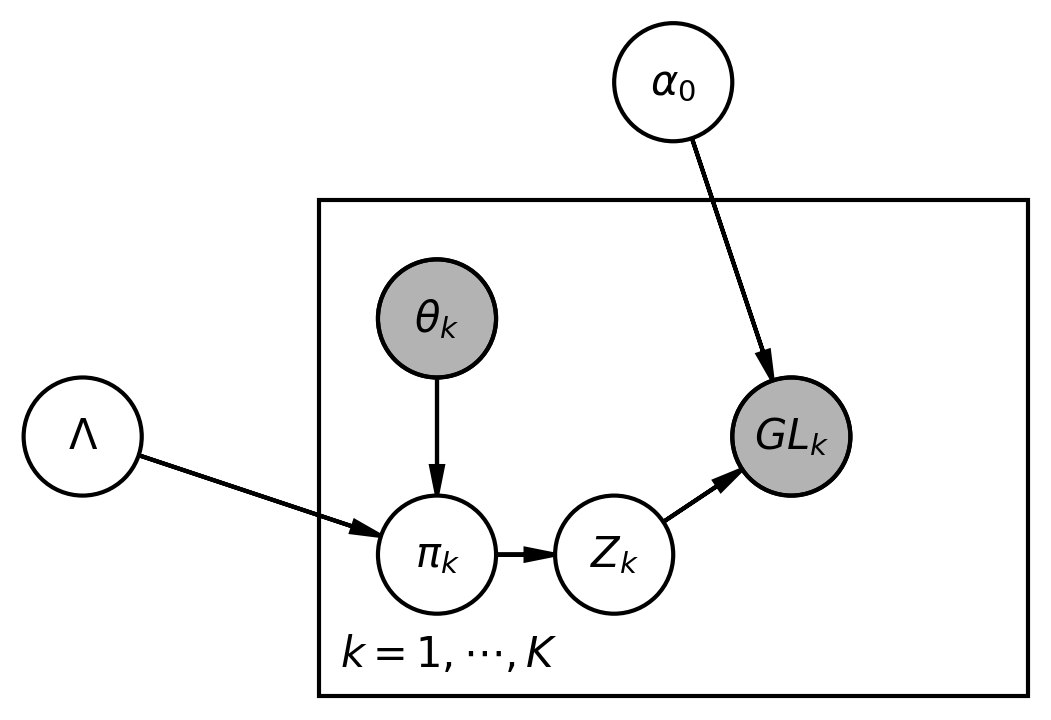
\includegraphics{figs/pGermlinePoly.model.png}
\end{center}
\caption{Graphical model representation of }
\end{figure*}


\section*{Model Validation}






\bibliographystyle{unsrt} % We choose the "plain" reference style
\bibliography{refs} % Entries are in the refs.bib file


\end{document}
